\documentclass{MScthesisITEM}

\title{Traffic data processing using\newlinetitle large scale graph processing} % The title of your assignement; NB use \newlinetitle to start a newline
\author{Yorin Anne de Jong} % Your firstname and lastname
\professor{Yuming Jiang, ITEM} % Affiliation = ITEM for instance
\supervisor{Gurvinder Singh, UNINETT}

%% Uncomment the following in case you want subfigures; note that there will be a warning for the caption package
% \let\subcaption\undefined
% \let\subfloat\undefined
% \usepackage[bf]{caption}
% \usepackage{subcaption}
\usepackage{lscape}

\DeclareGraphicsExtensions{.pdf,.jpg,.png}
\graphicspath{{./figs/}}

\loadglsentries{glossary}
\makeglossaries

\begin{document}
\selectlanguage{english}
\pagenumbering{roman}
\pagestyle{plain}

%% Only for the project
%\titleITEM

%% Only for the master's thesis; for the project report the description is taken from It's Learning and added by the department
\selectlanguage{english} % Change to 'norsk' if you are writing in Norwegian
\begin{titlingpage}

\noindent
\begin{tabular}{@{}p{4cm}l}
\textbf{Title:} 	& \thetitle \\
\textbf{Student:}	& \theauthor \\
\end{tabular}

\vspace{4ex}
\noindent\textbf{Problem description:}
\vspace{2ex}

\noindent 
Computers connected to the internet are subject to being infected with different kinds of malware.
Often, an infected computer will try to infect more computers, launch attacks, send spam or produce other malicious traffic.
The general scope of the thesis work is to investigate method(s) to automatically detect such malicious traffic from large datasets (e.g. in the order of hundreds of gigabytes of metadata) by means of anomaly detection.
The specific goal of the thesis work is to investigate different methods to store NetFlow data in a scalable graph structure, and subsequently try different graph processing systems on the NetFlow data to detect malicious traffic.
It is expected that the work will use at least one of the available graph processing frameworks to detect malicious traffic on the network.
NetFlow data is provided by UNINETT and consists of metadata of traffic but not payload (e.g. the fact that two IP addresses exchanged packets, but not their contents).

\vspace{6ex}

\noindent
\begin{tabular}{@{}p{4cm}l}
\textbf{Responsible professor:} 	& \theprofessor \\
\textbf{Supervisor:}			& \thesupervisor \\
\end{tabular}

\end{titlingpage}

\cleardoublepage

%% There must be an abstract in English, even though the main text is in Norwegian
\selectlanguage{english}
\pagestyle{empty}
\begin{abstract}
\noindent Anomaly detection in internet traffic today is largely based on quantifying traffic data.
This thesis proposes a new algorithm SpreadRank,
 which detects spreading of internet traffic as an additional metric for traffic anomaly detection.
SpreadRank uses large scale graph processing to calculate spreading from multiple gigabytes of NetFlow data obtained from core routers.
Studying spreading is a useful tool in determining the role of an end-host and in identifying malicious behaviour.
\end{abstract}

\cleardoublepage

%% Only for the master's thesis; if the main text is in English and you can write Norwegian, there must be an abstract in Norwegian as well.A
\selectlanguage{norsk}
\pagestyle{empty}
\renewcommand{\abstractname}{Sammendrag}
\begin{abstract}
\noindent Anomalideteksjon i nettrafikk i dag er stortsett basert på mengder trafikk.
Denne avhandlingen introduserer en ny algoritme SpreadRank,
 som vil detektere spredning i nettrafikk som et ekstra målepunkt for anomalideteksjon.
SpreadRank vil bruke flere gigabytes i NetFlow logg fra core-rutere i storskala grafprosessering for å beregne spredning.
Spredning er et nyttig verktøy for å undersøke hva slags rolle en datamaskin på nettet har og for å finne skadelig oppførsel.

\end{abstract}
\cleardoublepage

\selectlanguage{english}% Change to 'norsk' if you are writing in Norwegian

\renewcommand{\abstractname}{Preface}
\begin{abstract}
\noindent PREFACE
\end{abstract}
\cleardoublepage

% similarly you may add a separate acknowledgments page

\tableofcontents*
\cleardoublepage

%% include if relevant
\listoffigures
\cleardoublepage

%% include if relevant
%\listoftables
%\cleardoublepage

%% include if relevant
\listofalgorithms
\addcontentsline{toc}{chapter}{List of Algorithms}
\cleardoublepage

%% include if relevant
\printglossary[title=List of Terms, style=long]
\cleardoublepage
\glsaddall[]

%% include if relevant
\printglossary[title=List of Acronyms,type=\acronymtype] % prints just the list of acronyms
\cleardoublepage

\pagenumbering{arabic}
\pagestyle{ruled}
\chapter{Introduction}
\label{chp:introduction} 

The internet today is a very important communication network.
Nearly everybody is connected to it, many are dependent on it,
 and the possibilities are virtually endless.
The applications range from looking at pictures of cats, to high intensity stock trading and remote surgeries;
however, not all applications are well intended towards other internet users.
Criminals write malware that will send spam and spy on people's computers to look for credit card information.
Activists use botnets to bombard sites they don't like, in order to make them unavailable.

Internet providers want to block clients that participate in harmful activity,
 but this is not a simple task.
The amount of traffic that passes through a back bone router is huge,
 and special provisions need to be in place to log this.
Cisco is a large supplier of router hardware, and has introduced the NetFlow format~\cite{cisco0netflow}.
NetFlow data does need to be stored an processed, for which multiple solutions are available~\cite{zaharia2010spark,Morken352472}.

Current software for analysing NetFlow logs is based on counting flows.
A relatively high number of flows in a short period of time is reason for alarm,
 and a high number of flows for a single IP address may be a reason to investigate.
The challenge is that a high number of flows does not necessarily indicate a problem.
% which may lead to false positives, which may lead to the raising of the minimal amount of flows for alarm.


\section{Anomaly detection}
An anomaly is a non-conforming pattern~\cite{Chandola:2009:ADS:1541880.1541882}.
There are multiple methods to detect anomalous traffic.
%Different devices on a network generate traffic for many different reasons.
%Some traffic is benign, some traffic is malicious.
%Some examples of are: \emph{web browsing}, \emph{e-mail}, \emph{software updates}, \emph{torrents}, \emph{VPN tunnels}, \emph{SSH tunnels}, \emph{port scans}, \emph{spamming}, \emph{(D)DoS attacks} and \emph{infecting other hosts}.
%However, when observing network traffic, the only kinds of anomalies that can be observed from first glance are
It is possible to detect high or low resource consumption~\cite{lan2003effect}, standards-conforming or non-standards-conforming packets~\cite{john2008detection}, or asymmetric traffic which should be symmetric~\cite{kreibich2005using}.
However, these anomalies do not necessary indicate malicious activity.
Non-standard packets may be sent between hosts running legacy and/or proprietary software,
asymmetric traffic may be caused by network scanning tools, improperly configured firewalls or IP spoofing,
and high-rate traffic can just as well indicate a popular server, as an attack~\cite{gao2006differentiating}.

%This thesis introduces the SpreadRank algorithm,
% which will provide additional metrics to judge an IP address on.
%It will use NetFlow data to determine if traffic is repeated by other hosts,
% in other words, when a host receives a connection, it will see if this host starts initiating the same kind of connection to other hosts.
This thesis will focus on spreading of traffic as an anomaly, as malicious traffic is intended to spread as far as possible,
 while bona fide traffic will often remain between two hosts.
To illustrate: a criminal who created malware that steals credit cards wants it installed on as many computers as possible.
The owner of a botnet wants as many computers as possible to join it.
An end user sending an e-mail or doing online banking, however, will want this information to be only available to the intended recipients.


\section{Graph processing}
Graph processing is often associated with data mining, due to Facebook actively working on the technology to mine social data~\cite{ching2013scaling},
 though it has a lot of different uses.
Some examples of graph processing in real-world applications are navigation (roads as edges), financial (currency flow), internet search (Google pagerank~\cite{page1999pagerank}) and rumour spreading~\cite{nekovee2007theory}.
This thesis will use graphs to process network data from NetFlow, which is a graph that shows information flow.

The NetFlow data will be provided by UNINETT, which administers the core routers in the Norwegian academic network.
Backbone NetFlow traffic is typically hundreds of megabytes to gigabytes of flow data per day.
By observing such a large network, it is possible to look for patterns.
Observing individual network nodes may give some indication of the type of traffic being sent,
 though observing the interaction between many different hosts can show information that is not visible by only observing a few hosts.


\section{Privacy}
This thesis is based on sampled NetFlow data from December 2013, made available by UNINETT.
NetFlow data contains, among others, source IP, destination IP, protocol, and time, but no payload information.
Sampled NetFlow is a NetFlow log where not everything is logged, UNINETT logs about~1~\% of flows, this is done for performance and storage reasons.
Even though no payload information was made available for this study, payload information can be helpful when identifying traffic.
There are known techniques for using payload information without infringing on privacy~\cite{parekh2006privacy}.


%\section{Previous work}
%Earlier research has focussed on the MapReduce model for processing graph data~\cite{Morken352472}.
%
%
%A similar study compares computer viruses to biological viruses~\cite{pastor2001epidemic},
% it focuses on the spread/recovery rates of computer viruses.
%The study does not focus on graph based systems
%This study will not focus on virus infections, but it will look at the spreading of traffic on the internet.
%

% "Hadoop~\cite{Borthakur:2011:AHG:1989323.1989438}"


 % introduction
\chapter{NetFlow}
\label{chp:netflow}

\section{Format}
The traffic data provided by UNINETT is stored in the NetFlow File Format~\cite{cisco0netflow}.
This format consists of flows, which are data units consisting of information from the \gls{network layer} and \gls{transport layer},
 for example IP addresses, transport protocol, and port numbers where applicable.
NetFlow can be converted to human readable text using the \verb"nfdump" program\footnote{\url{http://nfdump.sourceforge.net}}.

\section{Available information}
%Apart from multicast and broadcast flows, flows are always between two hosts.
%The NetFlow information is logged by UNINETT's core routers, so only traffic that passes through these core routers is logged.
%Flows that are not logged are (1) communication in LANs and (2) communication on the open internet between hosts that have no affiliation with UNINETT.
%This means that (1) spreading of malware within a LAN, or organisation, is not detected and neither is (2) malware spreading on the internet outside of the Norwegian academic institutions.
%
%Using a list of IP addresses assigned to UNINETT and organisations peering through UNINETT, it is possible to know which hosts can be well observed (all communication with the internet is observed) and which %hosts cannot be well observed (only communication with a well observed host is observed).
%The thesis focuses mainly on hosts that can be well observed.
%
%\subsection{Observable traffic}
NetFlow data is logged on the core routers, which means that only traffic that passes through these routers is observable.
UNINETT peers with most Norwegian education institutions, which have their own routers connected to the core routers.
This means that UNINETT can only observe traffic that happens between institutions, or between institutions and hosts on the outside.
In other words, traffic between hosts within an institution is not observable for UNINETT.
%Although there exists malware with very specific targets~\cite{langner2011stuxnet}, most known malware targets any vulnerable host on the internet it can find.
%Because of this, it is expected that most malware traffic will be observable from the NetFlow data.

Figure~\ref{fig:nodes} shows some hosts in different networks, and some flows between them.
The figure illustrates how only flows that go through UNINETT's core routers will show up in the NetFlow log.
Flows between hosts within an institution will never pass through UNINETT's core routers, even though the institution is connected to the internet through UNINETT.
Flows completely outside of UNINETT's core network are not logged either, naturally.
Flows that are between one host at an institution connected through UNINETT -- for example \gls{ntnu} -- and one host in another institution, can be logged by UNINETT's core routers, because the traffic must pass through these routers.

\begin{figure}[h]
	\caption{Illustration of which flows are logged}
	\label{fig:nodes}
	\centering
		\includegraphics[width=0.5\textwidth]{nodes}
\end{figure}


\section{Direction}
\label{sec:direction}

Flows are between a source and destination IP address.
One TCP or UDP session will usually be observed as multiple flows,
because NetFlow logs are written by core routers operating on the \gls{network layer},
 which will not keep track of TCP of UDP connections, as this is a \gls{transport layer} function.
In order to observe spreading, it is important to know which host initiated the connection.
A possible solution would be to take the first flow between two hosts, and merge it with all subsequent flows that are between the same IP addresses and port numbers,
 until a time-out occurs.
However, for performance reasons, UNINETT makes use of sampled NetFlow data, which means that only 1~\% of all the packets are logged.
This makes it harder to reliably establish which party initiated a connection,
 as the first observed flow may be in the opposite direction from the actual first flow.

TCP and UDP are transport protocols which offer end-to-end communication between hosts.
In order to allow hosts to run multiple services, these protocols use a two byte \emph{port number} to indicate the type of service.
In order to set up a TCP or UDP connection, a client must first select a port number at random.
This port is called the \emph{\gls{ephemeral port}}, and its range differs per operating system, but it is never lower than 1024.
The client will then send an initial packet to the server, from the \emph{\gls{ephemeral port}}, to the \emph{\gls{contact port}}.
The \emph{\gls{contact port}} will often be a \emph{\gls{well-known port}}, which is a port number under 1024.
The direction of a flow can therefore be assumed to be initiated by the party with the lowest port number.
The list of \gls{well-known port}s is maintained by IANA~\cite{rfc1700}.


 % description of the NetFlow format
\chapter{Graph processing}
\label{chp:graph}

In order to process large graphs, a graph processing system is required.
A graph processing system uses a data model of vertices which are connected by edges~\cite{sakr2013processing}.
Vertices can have an ID and a value, edges can have a direction and a value.
The vertex values are modified during computation, and edges can be added and/or removed during computation.
A graph system can scale out horizontally (linearly with size), and is therefore able to process graph data at large scale.
A large graph system must also be able to handle failover, such as network, storage or hardware failure.
There are multiple graph systems available,
 for example GraphLab~\cite{low2010graphlab}, 
 GraphX~\cite{xin2013graphx}, 
 Pregel~\cite{Malewicz:2010:PSL:1807167.1807184} 
 and Giraph~\cite{avery2011giraph,ching2013scaling}.
This thesis will focus on Giraph,
 but other systems are expected to give similar results.

\section{Bulk Synchronous Parallel model}
\label{sec:bsp}

\begin{figure}[h]
	\caption{BSP programming model~\cite{sakr2013processing}}
	\label{fig:BSP}
	\centering
		\includegraphics[width=1\textwidth]{BSP}
\end{figure}

By running calculations in parallel, more computations per second are possible.
The case for parallel computing is strengthened by the fact that processing power is cheap nowadays,
 but fast processing is achieved by using many processors in parallel.
Parallel computing does, however, pose an important challenge,
 in that a single processor cannot share memory with another processor, and synchronisation is expensive,
 as it requires processors to wait, as memory cannot be reliably changed by two different processes.

The Bulk Synchronous Parallel model~\cite{Valiant:1990:BMP:79173.79181} (figure~\ref{fig:BSP}) is a model for parallel computing.
It consists of components that handle processing and/or memory.
Operations are divided in so-called supersteps.
A router allows components to exchange point to point messages at the end of a superstep execution,
 which allows for storage access between components.
The model is useful for running large calculations that will take a very long time with standard hardware.

\section{Giraph}
Giraph is a software based implementation of the the Bulk Synchronous Parallel model,
 and allows for a large amount of physical machines to form a cluster.
A Giraph computation program consists of a single \verb"calculate" function, which has two arguments; (1) the vertex and (2) the messages that were sent to the vertex during the last superstep.
During every superstep of the computation, a vertex may send a message to another vertex via one of its outgoing edges.
A vertex may also ``vote to halt'', to indicate that it is done calculating.
If a vertex votes to halt, it will not be called during subsequent supersteps, unless it receives a message from another vertex.
A vertex that has received a message will always be called, and any previous votes to halt are forgotten; the vertex will have to vote to halt again.

Before the computation is started, the graph is read by a \verb"VertexInputFormat" or an \verb"EdgeInputFormat".
After computation, the graph is written by a \verb"VertexOutputFormat" or \verb"EdgeOutputFormat"\footnote{\url{https://giraph.apache.org/io.html}}.
When the program is started, Giraph will start worker processes on the physical machines.
The workers will each read a part of the graph, Giraph will distribute the graph, workers will execute supersteps and after the last step is completed, the workers write their part of the graph.

Giraph takes care of the communication between the workers, and distributes the workload over the workers.
Due to the nature of BSP, it is important for Giraph that every worker will take roughly the same amount of time to complete a superstep.
After each superstep, the nodes have to synchronise and start working on the next superstep, which means that if one worker is slow, all other workers have to wait for it to finish.

\section{Design choices}
\subsection{Optimisations}
When implementing a computation for a graph system, such as Giraph, it is important to make the run-time of each computation as short as possible.
During each superstep, all workers will run computations, so that each vertex is computed once per superstep.
During a single computation, all incoming messages to the vertex for that superstep must be handled, and possibly all outgoing edges must be iterated over to send messages to neighbouring vertices.
Iteration is a weak spot for parallel systems, as it is not executed in parallel.
Therefore, in order to cut on computation time, vertices should have as few edges as possible.
%Section~\ref{sec:model_optimisation} describes how SpreadRank optimises the model.




% "*** Explain a bit how you have done and which choices you made in your thesis work."

 % description of the graph structure
\chapter{Traffic in a graph}
\label{chp:traffic}

The internet is a world-wide network where all hosts can communicate with each other.
Seen from a consumers' viewpoint, the internet is an outlet in the wall, or a wireless subscription.
Connecting to the internet will give instant access to any website in the world (figure~\ref{fig:graph-lay4}).
Seen from the viewpoint of a network engineer, it is a vast infrastructure with countless routers connected with countless wires (figure~\ref{fig:graph-lay3}).
Connecting to the internet is to peer with an ISP, which peers with other ISPs, etc.,
 making a global network where any host can communicate with virtually any other host.
These two definitions are both correct, but they describe the internet on a different layer in the OSI model.
The OSI model~\cite{zimmermann1980osi} is a model that partitions the internal functions of a communication system into abstraction layers.

\begin{figure}[h]
	\caption{A network observed on the transport layer; clients have direct contact to servers}
	\label{fig:graph-lay4}
	\centering
		\includegraphics[width=1\textwidth]{graph-lay4}
\end{figure}

\begin{figure}[h]
	\caption{A network observed on the network layer; all devices are interconnected via routers}
	\label{fig:graph-lay3}
	\centering
		\includegraphics[width=1\textwidth]{graph-lay3}
\end{figure}

The network layer describes how datagrams are routed between two hosts on the network.
This delivery is realised by routers between these hosts,
 where each router forwards datagrams to a router that is closer to the destination.
Datagrams are data packets, which start with an IP-header,
 which contains the source and destination IP address of the datagram.
IP-addresses are fixed-length numbers of 32-bits (IPv4) or 128-bits (IPv6).

The transport layer describes segments being sent directly between hosts,
 not considering any routers.
Typically, segments will have a protocol header, often TCP or UDP.
The TCP and UDP headers contain two 16-bit port numbers (source port and destination port),
which often indicate the kind of traffic in the packet.
For example,
 port 80 indicates web traffic,
 443 indicates encrypted web traffic,
 53 indicates DNS traffic and 22 indicates SSH traffic.


\section{Model optimisation}
\label{sec:model_optimisation}

A possible approach to implement the NetFlow data model as a graph, is to represent IP addresses as vertices, and a combination of (1) ports and (2) time as edges (figure~\ref{fig:graph-pragma}).
This model contains vertices with many edges, which could take a long time to calculate per superstep.
However, this model contains information that is not going to be used.
Removing this information will allow computation to speed up, as unnecessary information will not take up computation time.
In SpreadRank, the \emph{\gls{ephemeral port} number} is not important,
 so it can be discarded.
Because SpreadRank will only look for \gls{spreading} over identical port numbers (using port numbers as a metric for same-type communication),
 the vertices can be split.
The result is a model in which a client that requests a DNS record and then a website will be represented by two vertices;
 one for the DNS client and one for the HTTP client.
The model is inaccurate when compared to real-world TCP or UDP, in that the source port and the destination port are equal
 (whereas in the real world the connections initiated from the client would be initiated from an \gls{ephemeral port}),
 but this model will make it easier to detect \gls{spreading} over identical ports, as will be explained in chapter~\ref{chp:spreadrank}.

\begin{figure}[h]
	\caption{Graph with IP as vertex, ports and time as edge}
	\label{fig:graph-pragma}
	\centering
		\includegraphics[width=.75\textwidth]{graph-pragma}
\end{figure}

Figure~\ref{fig:graph-optim} shows the optimised version of figure~\ref{fig:graph-pragma}.
There will not be any edge from a DNS vertex to a HTTP vertex.
This will make it easier for Giraph to distribute the graph over different workers,
 in such a way that no vertices need to be moved in between supersteps.

\begin{figure}[h]
	\caption{Graph with IP and port as vertex, time as edge}
	\label{fig:graph-optim}
	\centering
		\includegraphics[width=.6\textwidth]{graph-optim}
\end{figure}


\subsection{Data conversion}
\label{sec:conversion}
In order to convert NetFlow to a graph in Giraph,
 an \verb"InputFormat" for NetFlow data must be devised.
Giraph has standard abstract readers and writers available that work with text formats.
For easier implementation, a \gls{bash} script was created that uses \verb"nfdump" to convert NetFlow to \gls{csv} files,
 and a Giraph \verb"EdgeInputFormat" was implemented that reads these \gls{csv} files.

The script filters its output so that only TCP and UDP flows remain where at least one port number is under 1024.
It will invert flows where the source port is the lowest port.
The script passes all its arguments to \verb"nfdump".

The recommended way to use this script is to convert NetFlow logs by day,
 so that multiple Giraph workers can read the graph at the same time.
This will not only speed up reading, but it may prevent a worker crashing from reading a too large file, since the graph is stored in memory.

Using \verb"nfdump" is not ideal, a better solution would have been to use a \verb"NetFlowInputReader" in Giraph directly.
At the time of writing, such a reader was not available.
It is beyond the scope of this thesis to write such an input format reader.

\begin{landscape}
\begin{verbatim}
	#!/bin/bash
	nfdump "$@" -o 'fmt:%ts %te %sa %da %pr %sp %dp %sas %das %in %out %tos %flg' | while read \
	    flowstartdate \
	    flowstarttime \
	    flowenddate \
	    flowendtime \
	    srcaddr \
	    dstaddr \
	    proto \
	    srcpt \
	    dstpt \
	    REST
	do
	    if [ "${proto}" = "TCP" -o "${proto}" = "UDP" ]
	    then
	        if [ "$srcpt" -lt 1024 -a "$dstpt" -ge 1024  -o  "$srcpt" -ge 1024 -a "$dstpt" -lt 1024 ]
	        then
	            [ $srcpt -lt $dstpt ] \
	                && echo $flowstartdate\ $flowstarttime,$dstaddr,$srcaddr,$srcpt \\
	                || echo $flowstartdate\ $flowstarttime,$srcaddr,$dstaddr,$dstpt \\

	        fi
	    fi
	done
\end{verbatim}
\end{landscape}


\section{Spreading}
Most hosts on the internet are either configured as a client or as a server, but some hosts are configured as both.
A server is, for the purpose of this analysis, defined as a host that will receive connections.
A client is, for the purpose of this analysis, defined as a host that will initiate connections.
A connection is thus always initiated by a client, but it allows two-way communication, which allows client and server to exchange information.

This model is based on the assumption that most home users (``clients'') will not run permanent services on their machines,
 but they will use e-mail and browse the web, which they do by contacting servers.
In some cases, however, home users may choose to run servers on their own equipment as well.
This can, for example, be a cheap solution to host a website or a mail server, or it can be done out of curiosity.
On the other hand, servers may themselves be clients, either temporary, for example during maintenance, or as mode of operation, for example a slave DNS server.

In some cases when a client initiates a connection to a server,
 the server may relay this connection to another server, or it may open a similar connection to another server.
This happens for example for proxy servers, which are configured to simply relay information.
Another example is a DNS resolver, which may be queried for a record in the global domain name system.
If it does not have this record available, it will query an authoritative server.

Spreading may also indicate the spreading of malware, for example a computer worm~\cite{pastor2001epidemic}.
By looking at how far traffic spreads and which port number it uses,
 it is possible to get an insight of what happens in the network.
This may prove helpful for finding infected machines in the network.

 % how NetFlow traffic can be represented as a graph
\chapter{Anomalies}
\label{chp:anomalies}


This thesis will propose the SpreadRank algorithm,
 which will detect traffic spreading on OSI layer 4.
What this means, is that it will detect end-hosts (clients and servers) that initiate the same kind of connections that they receive.
The discriminator used to identify same-kind connections is the \gls{contact port} number associated with a flow.
The assumption is that a service both receiving and initiating connections to the same port is an anomaly.
For example, a workstation with a web browser and e-mail client will initiate connections to ports 80 (HTTP), 443 (HTTPS), 587 (SMTP submission) and 143 or 993 (IMAP and IMAPS respectively).
However, it is not expected that such a workstation would \emph{receive} connections towards these port numbers.
Neither is it expected that the web server would initiate connections directed towards port 80 or 443.

This is not true for all protocols.
For example, a mail server can forward e-mail to another mail server via port 25 (SMTP),
 and this second mail server may forward it to a third mail server over port 25 and so forth.
There are several other protocols that exhibit natural spreading, these are described in section~\ref{sec:proto_spreading}.



\section{Servers undergoing maintenance}
\begin{figure}[h!]
	\caption{Observed spreading caused by a server under maintenance}
	\label{fig:spread_maintenance}
	\centering
		\includegraphics[width=0.5\textwidth]{spread_maintenance}
\end{figure}
Figure~\ref{fig:spread_maintenance} shows spreading caused by a server undergoing maintenance.
A server undergoing maintenance may connect to another server,
 for example to get the latest software updates.
Additionally, there exists server software that includes a graphical user interface,
 which gives the server the same look and feel as a workstation.
On these servers, the administrator may be inclined to use a web browser to download software or even browse the web.


\section{Home connections which run a personal server}
\begin{figure}[h!]
	\caption{Observed spreading caused by a single home server}
	\label{fig:spread_home}
	\centering
		\includegraphics[width=0.5\textwidth]{spread_home}
\end{figure}

Figure~\ref{fig:spread_home} shows spreading caused by servers run by home users on a shared public IP address.
Users with a home server will often run the home server on the same IP address as the client.
This is done either by simply using the same machine as server and client,
 or by using a NAT router, allowing a separate client and server machine to share a public IP address.
When a client and a server share an IP address, this IP address will generally both receive and initiate flows.
Since there is no direct way to distinguish whether incoming and outgoing flows are related,
 such a situation might register as a case of spreading.
However, home servers are quite common, but a trail of home users with servers contacting each other can show up as an anomaly.


\section{VPN servers}
\begin{figure}[h!]
	\caption{Observed spreading caused by a VPN server}
	\label{fig:spread_vpn}
	\centering
		\includegraphics[width=0.5\textwidth]{spread_vpn}
\end{figure}

Clients can set up a secure connection to a VPN server (figure~\ref{fig:spread_vpn}).
All internet traffic initiated at the client (apart from the VPN traffic itself) will be sent to the VPN server in encapsulated form.
The VPN server removes the encapsulating, and forwards the traffic towards the internet, possibly mimicking a client.
Thus, if the client tunnels another VPN connection through the VPN server, the VPN server may appear to be a VPN client as well.

Some providers allow using SSH, HTTP or HTTPS for VPN.
Examples of software that can do this are sshttp~\cite{github:stealth:sshttp} and Microsoft RRAS~\cite{rras}.
When a user connects to a VPN server over HTTPS, and then uses the VPN to connect to a HTTPS host, this can register as spreading.
However, some VPN servers allocate dedicated public IP addresses to their clients,
 which means that connections are not forwarded over the same IP, which means that the VPN does not register as spreading.


\section{Protocols with natural spreading}
\label{sec:proto_spreading}
\subsection{BGP}
BGP is a protocol used by routers to exchange routing information.
Even though routers are level three devices themselves, they exchange routing information with each other the same way end-hosts do.
Routers both listen for incoming BGP connections, and send BGP to neighbouring routers at regular intervals.
Since routers both receive and initiate BGP flows, BGP spreading is expected to be high.

\subsection{DNS}
Clients use DNS to find the IP address associated to a hostname.
If the DNS server does not have the record in its cache,
 it must forward the query to an upstream server,
 or find the authoritative DNS server for that host and forward the query there.
Forwarding DNS is expected to cause high spreading.


\subsection{SMTP}
Most e-mail clients are configured with a so-called ``smart host'',
 which is the server that all outgoing mail is sent to.
This smart host will then find out which server handles e-mail for the recipient, and forward the message there.
In some cases, the e-mail will pass multiple servers before finally reaching a mailbox.
Naturally, this means that some spreading in the SMTP protocol is expected.


\section{HTTP/HTTPS}
\label{sec:http}
A large number of different services use HTTP and HTTPS as underlying layer for their data.
SpreadRank may therefore observe trails of machines connecting over port 80 or 443,
 without these flows actually being related.
There is currently no direct way to view the difference between different services provided over HTTP or HTTPS, purely based on NetFlow data.

%Possibly less clear cases of spreading are \gls{SSH} and \gls{HTTP}.
%Although these protocols are meant for client-server communication (\gls{SSH} allows clients to connect to a remote shell, \gls{HTTP} is the protocol used for web pages),
% it is possible that a user will use the SSH session to another SSH server from there.
%A proxy web server can request a page on its clients behalf.
%These services yield low depths, as most servers providing these services will not forward information they receive.


\section{Combination}
\begin{figure}[h!]
	\caption{Observed spreading caused by a combination of benign factors}
	\label{fig:spread_combi}
	\centering
		\includegraphics[width=0.75\textwidth]{spread_combi}
\end{figure}

A combination of different occurrences of spreading may lead to larger spreading, as shown in figure~\ref{fig:spread_combi}.
However, the depth, is still relatively limited.
This means that relatively short paths are not anomalies.
%From which length spreading becomes an anomaly depends on the protocol and the size of the NetFlow dataset,
% but from the results of the experiment, 20-30 steps seem like a reasonable amount.
%Because of this, if only a single host is observed generating the same kind of traffic as it receives, no conclusions can be drawn from that.
%However, if there is a long trail of hosts sending the same kind of traffic, there is a good chance that this is a worm at work.


\section{Worm infection}
A worm is a piece of software that is programmed to infect other hosts in such a way that these hosts will run the worm, too.
It infects a host by looking for systems that run unpatched software,
 and using a known security hole to get access to the service and install itself.
After infection, the victim will start doing the same.
This process can go on for ever, until a system administrator starts blocking these flows.
Consequently, a worm that successfully spreads over many end-hosts, will show large spreading.


\section{Peer to peer traffic}
Peer to peer traffic is another case of spreading that happens intentionally;
a hallmark example is BitTorrent.
BitTorrent is a protocol for distributed file sharing, where all clients will make chunks they have downloaded available to other clients.
This differs from the traditional client/server model, where clients do not spread information to other clients but get all their information from a central server.
BitTorrent, however, operates over many different port numbers, which makes it difficult to match incoming and outgoing flows together.

The same is true for Tor traffic.
Tor is a mechanism for anonymous internet access, which works by encrypting traffic and routing it at random through multiple hops,
before sending it to the final destination.
Tor also operates on random ports, which makes it difficult to match flows together.

\subsection{Stealth worm}
Due to BitTorrent and Tor being able to hide their activity from an algorithm as SpreadRank,
the question arises whether a worm can do the same thing to hide its activity.
The important difference between benign traffic, such as BitTorrent and Tor, and malicious traffic such as worms,
is consent from the owner of the host.
If a host is participating in BitTorrent or Tor, it is because the owner of the host voluntarily installed software to supports these protocols.
Because these protocols can rely on software being installed, they can use virtually any connection model imaginable.

This is different for malware;
the initial infection must happen through a known vulnerability in the host.
This vulnerability will typically be part of the operating system or some type software that is installed.
Malware has therefore limited possibilities for infection, and must follow the specification of the software it wants to attack, which will often run on a standard port.
Thus, in order to attack a specific service, malware must target the same port for every attack.

Once a host has been infected, the malware can install itself, and it may communicate with command-and-control servers through stealth communication channels that may not be as easy to detect.
However, it will in all likelihood still try to attack other hosts, to increase the amount of infected hosts, for which it will have to generate observable traffic, for reasons mentioned earlier.



 % possible anomalies
\chapter{DOSRank}
\label{chp:dosrank}

To test Giraph, two simple algorithms, DOSRank and ReverseDOSRank are created, which count the amount of respectively incoming and outgoing edges from or to a vertex.
This proof of concept will count the amount of flows per \gls{service}.
It can be used to detect if a machine is executing or suffering from a DoS attack,
 as these are typically identified by a large number of flows.
These two algorithms will count respectively the amount of outgoing and the amount of incoming edges.
DOSRank (equation~\ref{eq:dosrank}, algorithm~\ref{alg:dosrank}), which will calculate outgoing edges (incoming connections) is trivial; it will set its value during the first superstep and vote to halt.
ReverseDOSRank (equation~\ref{eq:reversedosrank}, algorithm~\ref{alg:reversedosrank}) is a bit more complex;
 since incoming edges are not visible in Giraph, the first superstep is used to send a message over every edge.
During the second superstep, every vertex will receive an amount of messages that is equal to its amount of incoming edges.


\begin{equation}
	\label{eq:dosrank}
	f(x) = N^{-}(x).
\end{equation}
\begin{equation}
	\label{eq:reversedosrank}
	f(y) = N^{+}(y).
\end{equation}

\begin{algorithm}[H]
	\label{alg:dosrank}
	\caption{DOSRank}
	\begin{verbatim}
	result = vertex.getNumEdges();
	vertex.voteToHalt();
	\end{verbatim}
\end{algorithm}
\begin{algorithm}[H]
	\label{alg:reversedosrank}
	\caption{ReverseDOSRank}
	\begin{verbatim}
	if superstep = 0 then
	begin
	    result = 0;
	    sendMessageToAllEdges();
	end
	else
	begin
	    while(messages.hasNext)
	    do
	        message.next();
	        result++;
	    end;
	    vertex.voteToHalt();
	end.
	\end{verbatim}
\end{algorithm}

\section{Expected results}
The algorithm will find IP addresses that are associated with large amounts of flows.
Opening a large amount of flows is different from sending large amounts of data,
 as sending a large amount of data is often a completely legitimate thing to do:
For example, sharing files via peer-to-peer protocols or serving large files over HTTP.
A large amount of flows, however, may be an indication that something is amiss.
It can indicate port scanning, or even targeted attacks like SYN flooding.
However, a large amount of flows can also simply indicate a very active or popular host.

\section{Purpose}
These algorithms are just a proof-of-concept to show that graph systems can be used for traffic analysis.
The algorithm itself is most likely easier to implement using other systems.
A simple MapReduce algorithm could probably yield the same results a smaller amount of time~\cite{Morken352472}.
However, this algorithm does show that Giraph can be used for traffic analysis,
 and it opens the door for more complex algorithms, like SpreadRank.


 % DOSRank proof of concept
\chapter{SpreadRank}
\label{chp:spreadrank}

The previous algorithm, DOSRank, calculated the amount of flows.
While a large amount of flows may indicate that something is wrong,
 it may also simply indicate a very active node.
This chapter proposes SpreadRank, an algorithm to find hosts that are standing out due to the spreading they are causing.
SpreadRank calculates how far connections spread.
Spreading as an anomaly is described in chapter~\ref{chp:anomalies}.


\section{Overview of algorithm}
This thesis proposes SpreadRank, an algorithm to determine how far similar traffic spreads over hosts.
\emph{depth} in SpreadRank is defined in equation~\ref{eq:spreadrank1} and illustrated in figure~\ref{fig:spreadrank}.
The value of $d$ is the longest path from a host initiating a connection to another host receiving a similar connection.
\emph{spreading} in SpreadRank is defined in equation~\ref{eq:spreadrank2} and illustrated in figure~\ref{fig:spreadrank}.
The value of $s$ is the sum of all neighbours' $d$ value, plus the amount of neighbours.
Another way of looking at SpreadRank, is that during the first superstep, all nodes will send a token in the opposite direction of the flow.
This token contains the timestamp from the flow.
During all subsequent steps, all nodes that have received a token will send tokens again, but \emph{only to flows that have a lower timestamp than the token}.
\emph{Depth} is then defined as the last superstep during which tokens were received, and \emph{spread} is defined as the total amount of tokens received.


\begin{figure}[h]
	\caption{Small example graph with results of one node, all nodes are hosts}
	\label{fig:spreadrank}
	\centering
		\includegraphics[width=0.75\textwidth]{spreadrank}
\end{figure}
\begin{equation}
	\label{eq:spreadrank1}
	d(x) = 1 + \max_{y \in N^{-}(x)} d(y).
\end{equation}
\begin{equation}
	\label{eq:spreadrank2}
	\displaystyle s(x) = \sum_{y \in N^{-}(x)} d(y) + \left\vert{N^{-}(x)}\right\vert.
\end{equation}
\emph{Where $E$ is the set of all edges in the graph, $f(x)$ and $f(y)$ are vertex values and $N^{-}(x)$ is a set of all incoming edges from vertex $x$.}



SpreadRank bears similarities to Google's PageRank~\cite{page1999pagerank}.
Both algorithms use a graph model where vertices and edges represent real-world elements.
PageRank's model consists of web pages and hyperlinks and
 SpreadRank's model consists of services and flows.
Both algorithms calculate values for vertices based on how they are connected to other vertices.
The algorithms do, however, calculate different things,
 and as such use different metrics for calculating vertex values.
This is most apparent in that in PageRank vertices send each other part of their current score,
 while in SpreadRank vertices simply send the timestamp of a flow start.
This is because time is not important in PageRank; it does not matter who made a link first,
 while for SpreadRank it is important to know when a flow occurred,
 as spreading must occur in chronological order.


\section{OSI model}
The \gls{network layer} provides stateless communication between hosts, and can be used to observe which hosts communicate with each other by means of IP addresses.
Additionally, the IP header contains a protocol number, which gives some rough idea of the type of service.
The transport layer (layer 4) provides end-to-end communication, and can be used to observe what kind of services are being used, by looking at the protocol header.
Internet traffic consists mostly of TCP traffic, which makes TCP port numbers an interesting thing to look at.
SpreadRank only looks at TCP traffic, and assumes that identical port numbers indicate identical types of service.

SpreadRank must not be confused with the Dijkstra algorithm~\cite{dijkstra1959note},
 which can be used by layer 3 devices to find the shortest path between hosts.
SpreadRank operates on NetFlow data, which contains IP addresses of hosts and port numbers, which is layer 4 data.
The path that is observed is not a path via internet routers, but a path of hosts imitating each others behaviour.


\section{Data types}
\label{sec:data-types}
In the SpreadRank algorithm proposed in this thesis,
 IP-address and port number tuples are represented by vertices (figure~\ref{fig:datatype-spreadrank-vertex-id}).
The choice for this combination is due to \gls{spreading} occurring over the same port, which is the best NetFlow metric available to indicate type of traffic.
The vertex's value (figure~\ref{fig:datatype-spreadrank-vertex-value}) contains how far the traffic reaches (\gls{depth}) and how far their traffic spreads (\gls{spreading}).
Flows are represented by edges.
The edge has the flow start timestamp as value (figure~\ref{fig:datatype-spreadrank-edge}).


\begin{figure}[h]
	\caption{Data type of a SpreadRank vertex ID}
	\label{fig:datatype-spreadrank-vertex-id}
	\centering
		\includegraphics[width=1\textwidth]{datatype-spreadrank-vertex-id}
\end{figure}
\begin{figure}[h]
	\caption{Data type of a SpreadRank edge}
	\label{fig:datatype-spreadrank-edge}
	\centering
		\includegraphics[width=1\textwidth]{datatype-spreadrank-edge}
\end{figure}
\begin{figure}[h]
	\caption{Data type of a SpreadRank vertex value}
	\label{fig:datatype-spreadrank-vertex-value}
	\centering
		\includegraphics[width=1\textwidth]{datatype-spreadrank-vertex-value}
\end{figure}


\subsection{Filtering}
\label{sec:filtering}
Before calculation, all flows that do not represent a TCP or UDP connection are removed,
 as well as every flow not between a \gls{contact port} and an \gls{ephemeral port}.
Since the difference between a \gls{contact port} and an \gls{ephemeral port} may be vague,
 a \gls{contact port} is assumed to be a \gls{well-known port}, which is any port number below 1024~\cite{rfc1700}.
Any port from 1024 and up is assumed to be an \gls{ephemeral port}.
Different operating systems use different port numbers as \gls{ephemeral port}s,
 but no operating system uses ports under 1024 as \gls{ephemeral port}s (section~\ref{sec:conversion}).

Additionally, all double flows are removed, which means that there are always zero, one or two flows between two edges (no flows, one-directional, bi-directional).
For every vertex-pair, for every direction, the oldest edge is retained.
Since each edge has a timestamp as value, the edge with the lowest value is retained and edges with higher values are removed.


\subsection{Loop protection}
The removal of redundant edges is to provide a loop protection mechanism.
In a graph system, it is difficult to detect loops;
During calculation, only information about the vertex itself is known (outgoing edges, vertex id, vertex value, incoming messages).
It is not viable to include a trail of previous edges to the messages that are exchanged after the calculation;
 this would be expensive in terms of memory.

In the specific case of SpreadRank, this problem can be solved by only considering the first time a flow has been observed,
 and to ignore all subsequent occurrences (figure~\ref{fig:sequence1}).
If a host initiated a type of connection before it ever received it, it certainly did not initiate these connections because of the connection it received,
 and it is not a case of spreading (figure~\ref{fig:sequence2}).
Multiple hosts can initiate a connection before spreading occurs, in which case it is assumed that both are responsible (figure~\ref{fig:sequence3} and~\ref{fig:sequence5}).
It is possible that spreading is incorrectly assumed due to the log not observing a previous connection (figure~\ref{fig:sequence4}).
This can for example happen when logging started after the second host initiated a connection, but before the first host did.

\begin{figure}[h]
	\caption{Removal of duplicate flows}
	\label{fig:sequence1}
	\centering
		\includegraphics[width=0.5\textwidth]{sequence1}
\end{figure}
\begin{figure}[h]
	\caption{Spreading can only occur in sequence}
	\label{fig:sequence2}
	\centering
		\includegraphics[width=0.5\textwidth]{sequence2}
\end{figure}
\begin{figure}[h]
	\caption{Spreading with two clients and one server}
	\label{fig:sequence3}
	\centering
		\includegraphics[width=0.5\textwidth]{sequence3}
\end{figure}
\begin{figure}[h]
	\caption{Spreading with two clients and two servers}
	\label{fig:sequence5}
	\centering
		\includegraphics[width=0.5\textwidth]{sequence5}
\end{figure}
\begin{figure}[h]
	\caption{False positive spreading}
	\label{fig:sequence4}
	\centering
		\includegraphics[width=0.5\textwidth]{sequence4}
\end{figure}

\begin{equation}
	\label{eq:spreading}
	S = T_{\text{firstReceived}} < T_{\text{firstSent}}
\end{equation}


\section{Implementation}
\label{sec:implementation}
In Giraph, it is not possible for a vertex to enumerate its incoming vertices, only outgoing vertices are available.
For this reason, all direction edges are \emph{reversed} in the model, so that they point towards the \emph{initiator} of the traffic, not to the \emph{receiver}.
During the first superstep, all vertices will send a message over all outgoing edges (this message goes in the opposite direction of the original flow).
The message consists of the value of the edge, which is the time that the connection was attempted (section~\ref{sec:data-types}).
During all subsequent supersteps, all vertices that receive at least one message, will send one message over every outging edge \emph{that has a lower value than the highest value of any message received}.
The reason for this is that spreading must happen sequentally;
 when a host X sends to Y and then receives from Z, it is not a case of spreading.
it is a case of spreading when host X receives from Z and then sends to Y.



\begin{algorithm}[h]
	\caption{SpreadRank}
	\begin{verbatim}
	if superstep = 0 then
	    removeDoubleEdges();
	    for edge : outgoingEdges
	    do
	        edge.send(edge.value);
	    end
	end
	else
	begin
	    lastMessage = max(messages);
	    for edge : outgoingEdges
	    do
	        if edge.value < lastMessage
	        then
	        begin
	            edge.send(edge.value);
	        end
	    end
	end
	vertex.voteToHalt();
	\end{verbatim}
\end{algorithm}


\section{Expected results}

\subsection{Depth}
\label{sec:depth}
The amount of supersteps is expected to be relatively low, except for protocols that naturally exhibit spreading.
A high amount of supersteps indicates that the host has generated a type of network traffic that is also generated by the hosts it has sent this traffic to, and that this process has repeated itself over several unique hosts, forming a path.


\subsection{Spreading}
A high amount of incoming messages indicates that this host has initiated many connections.
This is typical behaviour for a client, and for protocols that have natural spreading (for example DNS resolvers and BGP).
Hosts that show high \gls{depth} (large amount of supersteps) but have a relatively small spreading,
 may be part of some internal group, where information spreads between members of the group, but not outwards.


\subsection{Clients}
The amount of clients is simply a count of the incoming edges, similar to DOSRank.
Since all edges are reversed (section~\ref{sec:implementation}),
 the amount of clients can simply be calculated by counting a vertex's outgoing edges in Giraph.
In the SpreadRank implementation written for this thesis,
 the amount is not calculated during a superstep, but simply included in the output while the results are written to disk.

%A host that has many outgoing connections (high spreading) that also has many incoming connections is probably just a very popular server.
A typical case where this value is useful, is for finding DNS resolvers.
Users (clients) of the DNS resolvers will typically have a higher \gls{depth} than the resolver itself,
 since the client initiated the connection (figure~\ref{fig:dns-clients}).
These clients themselves should have zero incoming connections, otherwise they are resolvers.

\begin{figure}[h]
	\caption{Illustration of how a single DNS resolver will have many incoming and outgoing connections.}
	\label{fig:dns-clients}
	\centering
		\includegraphics[width=0.5\textwidth]{dns-clients}
\end{figure}

By having the possibility to exclude vertices with few clients from the end results,
 it is trivial to limit the results to vertices with the second-longest path.
This will make it easier to focus on hosts that forward traffic, and not on hosts that only initiate traffic.

 % SpreadRank algorithm
\chapter{Results}
\label{chp:results}

UNINETT has provided NetFlow data over December 2013, in the NetFlow file format.
To simplify implementation, \gls{nfdump} was used to convert the flows to \gls{csv} files.
SpreadRank was run on the flows logged by one router over one day, one week, two weeks and one month.
Calculation of SpreadRank scores only took some minutes to complete,
 but the conversion to \gls{csv} took a few hours to complete.
This was likely due to the fact that \gls{nfdump} had to read the compressed NetFlow files from \gls{HDFS},
 and then write uncompressed \gls{csv} files onto the same HDFS volume.

After calculation, \gls{Giraph} writes output files containing all vertex IDs as values.
The vertex value (figure~\ref{fig:datatype-spreadrank-vertex-value}) consists of the depth and the spreading of the vertex.
A Giraph OutputFormat was implemented in order to make the output files better parseable using GNU utilities.

\section{Longest path}
Most \gls{service}s on the internet do not exhibit spreading.
Figure~\ref{fig:spreading-perstep-pie} shows a plot of spreading per vertex, calculated over NetFlow information from one router during one day and during one month.
Most vertices have a spreading of zero, one or two.
A spreading of zero typically indicates a server, one typically indicates a client (its traffic reaches to the servers) and a spreading of two often indicates a hybrid, but it can also indicate a simple proxy server.
Higher spreading indicates end-hosts that do participate in spreading.
This is typical for DNS servers, SMTP servers and BGP routers.

\begin{figure}[h!]
	\caption{Spreading per vertex}
	\label{fig:spreading-perstep-pie}
	\centering
		\includegraphics[width=1\textwidth]{spreading-perstep-pie}
\end{figure}

\section{Protocols}
After filtering traffic such that only \gls{service}s with a spreading of one or higher,
 and a depth of two or higher remain, only a few protocols remain (figure~\ref{fig:protocol-pie}).
This confirms the assumptions stated in section~\ref{sec:depth} and chapter~\ref{chp:anomalies},
 which is that spreading is expected to happen only on certain protocols.
\Gls{BGP}, \gls{DNS} and \gls{SMTP} are expected to spread, due to the way the protocols work.
\Gls{BGP} is used between routers to calculate shortest paths; routers need to keep each other updated and thus all will eventually initiate a connection,
 which might lead to another router relaying the information to other routers.
\gls{DNS} and \gls{SMTP} are both protocols where clients send their request to a server that is close to them,
 and the server will then handle the request.
In the case of \gls{DNS}, this means that the server will answer with information from its cache, or look the requested record up itself.
In the case of \gls{SMTP}, this means that the server will forward e-mail to the mail server of the recipient.
These services yield high depths, as virtually any server providing these services can forward information it receives.


\begin{figure}[h!]
	\caption{Distribution of protocols that exhibit spreading}
	\label{fig:protocol-pie}
	\centering
		\includegraphics[width=1\textwidth]{protocol-pie}
\end{figure}


The \gls{SSH} and \gls{HTTP} protocols also show up with higher spreading.
This may be due to home servers often serving web pages,
 and Linux-based home servers will typically also listen for SSH for remote management.
HTTP spreading is discussed in more detail in section~\ref{sec:http}.

Remarkable results are spreading on ports 666 and 445.
Port 666 is officially allocated as the port for computer game Doom~\cite{rfc1700},
 but in practice it is also used by viruses.
Only one instance of spreading over port 666 was observed over one month.
Port 445 is used by Microsoft Windows for sharing files, but it is also abused for denial of service attacks~\cite{lazarevic2003comparative}.
Because of this, it is unknown whether this spreading was due to an attack, or simply some users that had used Microsoft Windows File Sharing.

\section{Plot}
Individual observed services with a reach of one or higher are plotted in figure~\ref{fig:31day}.
It is based on one month worth of NetFlow.

\begin{itemize}
\item The X axis shows \gls{spreading} -- the amount of end-hosts reached via spreading -- the amount of messages received in total.
\item The Y axis shows \gls{depth} -- the longest path.
\item The size of the dot shows the amount of observed \gls{client}s -- the amount of incoming connections to the end-host.
\end{itemize}

\begin{figure}[h!]
	\caption{End-hosts scored with SpreadRank over one month}
	\label{fig:31day}
	\centering
		\includegraphics[width=1\textwidth]{31day}
\end{figure}

%The plots show a clear pattern.
%The pattern is not very clear in the plot from one day, but becomes clearer in the subsequet plots.
%The curve on the left side is simply an effect of the logarithmic scale of the plot;
% spreading can not be lower than the depth.
%The plot has an E shape, with many services with few clients at the low end of the spreading,
% and few services with many clients at the high end of the spreading.
%Each protocol in the plot has its maximum reach.
%The maximum reach is favoured by services with a high spreading, hence the E shape of the plot.

\section{Observed anomalies}
Figure~\ref{fig:31day} shows all observed IP-address + port number combinations with a depth of 2 or higher.
The best way to observe anomalies in this plot, is by Multi-class Anomaly Detection.
Multi-class classification assumes that the data set contains different distinct types of data~\cite{Chandola:2009:ADS:1541880.1541882}.
In the case of SpreadRank, these types of data are the port numbers.
Different ports are indicated with different colours in the plot, and it is apparent that there is a pattern.
It is also apparent that there are some outliers (figure~\ref{fig:spreadrank-pattern}, but there is no clear border between normal observations and anomalous observations.
However, a simple visual observation of the plot does give some interesting results.

\begin{figure}[h!]
	\caption{SpreadRank pattern over one month}
	\label{fig:spreadrank-pattern}
	\centering
		\includegraphics[width=1\textwidth]{spreadrank-pattern}
\end{figure}

\subsection{Botnet}
\label{ssec:botnet}

\begin{figure}[h!]
	\caption{HTTP and SSH traffic in SpreadRank over one month}
	\label{fig:31day-botnet}
	\centering
		\includegraphics[width=1\textwidth]{31day-botnet}
\end{figure}

Figure~\ref{fig:31day-botnet} shows \gls{HTTP} and \gls{SSH} services.
Dots marked with a solid line are linked to hosts that were reported to CERT.
The tiny red SSH node at the right hand side has been involved in \gls{SSH} scanning,
 where it connects to many IP addresses in the hope to find an SSH server with a password it can guess.
The large HTTP node at the right hand side was confirmed participating in a botnet during December 2013,
 but it was not discovered until January.
The host had many incoming and outgoing connections over port 80 in December, but at the moment of writing the host was down (no response).
After analysing the logs with more detail, it appeared that it was contacted very often by servers hosting questionable content.
These servers were contacted by various clients at the \gls{ntnu} at a regular interval,
 but starting the 24th of December, some of these servers started contacting the machine at \gls{ntnu}.
On January 1st, 2014, UNINETT CERT received a report stating that the machine participated in a botnet.

By matching the IP addresses this botnet host had contact with,
 two additional hosts were discovered participating in the botnet.
These two hosts were not reported to CERT, and were therefore never investigated.
Since none of the machines are up at the moment of writing this thesis,
 no further investigation is done.

According to information from \gls{DNS}, the host that got reported to CERT is a machine at a faculty at \gls{ntnu}.
The two hosts that were found using SpreadRank are computers at two different student villages at \gls{ntnu}.
More precise information is available at UNINETT at the time of writing, but cannot be published in this thesis for privacy reasons.

\subsection{DNS}
\begin{figure}[h!]
	\caption{DNS traffic in SpreadRank over one month}
	\label{fig:31day-dns}
	\centering
		\includegraphics[width=1\textwidth]{31day-dns}
\end{figure}

Figure~\ref{fig:31day-dns} shows \gls{DNS} services, marked by which institution manages them.
DNS resolvers are used to lookup DNS records for hosts inside the network.
These resolvers cannot be used from the outside, which is why the dots are small;
 the clients are inside the institution, and are therefore not logged by UNINETT's core routers (figure~\ref{fig:nodes}).

Authoritative DNS servers that cause spreading may seem like an anomaly;
 Authoritative DNS servers answer queries from clients and do not send queries themselves.
However, there is an explanation for this spreading:
In order to keep DNS zones available, most domains use multiple DNS servers.
These DNS servers must keep in sync, and will therefore periodically contact a master server if it is not itself the master for the DNS zone.


\subsection{SMTP}
SMTP is the protocol used for mail delivery, where sometimes an e-mail is forwarded a couple of times before it reaches a mailbox.
This causes spreading, which can be seen in figure~\ref{fig:31day}.
There are some SMTP services that have very high spreading, but these are simply hosts that handle high amounts of mail per day.


\section{Performance}
UNINETT made a server cluster available for the analysis.
This cluster is installed with Apache Hadoop~\cite{Borthakur:2011:AHG:1989323.1989438}, and consists of 15 worker machines with 4~CPUs and 16~GB RAM each.
In addition, there are two HDFS name-nodes and one YARN manager, which have 4~CPUs, and 10~GB RAM each.

Figure~\ref{fig:performance} shows how SpreadRank performs on this cluster,
 by NetFlow logs over one day, one week, two weeks and one month.
The logs are cumulative, so the one week log also contains the information from the one day log, etc.
Since every task is devided over multiple workers, of which multiple can exist on one worker machine,
 the calculation times fluctuate.
The figure shows one measurement where SpreadRank is run four times, for different NetFlow log sizes.
An interesting result is that the calculation of one week takes slightly longer than the calculation of two weeks.
This is probably by accident, the job may have been scheduled in such a way that multiple workers were located on the same physical machine.

\begin{figure}[h!]
	\caption{Time used to calculate SpreadRank}
	\label{fig:performance}
	\centering
		\includegraphics[width=.75\textwidth]{performance}
\end{figure}


\section{Comparison to other systems}
Software already exists to handle NetFlow logs.
The goal of most of this software is to make NetFlow logs easier readable.
UNINETT currently uses NFSEN\footnote{http://nfsen.sourceforge.net} for analysis of NetFlow information.
NFSEN provides a web interface from which the NetFlow log can easily be accessed as text or aggregrated plot (figure~\ref{fig:details-graphs}).
The aggregated data from NFSEN can be generated using MapReduce~\cite{Morken352472}.

\begin{figure}[h!]
	\caption{Screenshot of NFSEN (http://nfsen.sourceforge.net/details-graphs.png)}
	\label{fig:details-graphs}
	\centering
		\includegraphics[width=1\textwidth]{details-graphs}
\end{figure}

SpreadRank, as implemented in this thesis, does not provide any database storage, plot generation or user interfaces.
The plots shown in this thesis were created using modeling tools and spreadsheet software.
SpreadRank, instead, aggregates flows in a more recursive way, which gives additional metrics about end-hosts.
These metrics would be useful to integrate in NFSEN, but NFSEN in its current form does not support plugins.
Software similar to NFSEN is FlowViewer\footnote{http://sourceforge.net/projects/flowviewer/} and SiLK~\footnote{https://tools.netsa.cert.org/silk/}.

 % Findings (and performance)
\chapter{Conclusion}
\label{chp:conclusion}

This thesis has stated the current practices in traffic anomaly detection.
Current traffic anomaly detection is based on aggregating flows,
 or by identifying high-intensity traffic.
The thesis defines the concept of spreading,
 which describes the phenomenon of an end-host initiating the same kind of connections it receives,
 where same-kind refers to usage of the same TCP/UDP ports.
It is argued that spreading is uncommon for most protocols on the internet today, which makes it an anomaly.

The usage of graph systems is proposed as a means to measure spreading.
Multiple graph systems are available today, this thesis uses the Giraph system.
Using Giraph, NetFlow information provided by UNINETT is converted to a graph,
 where spreading is calculated using SpreadRank, an algorithm introduced in this thesis.

SpreadRank works by making a graph of flow data.
In this graph, vertices represent IP address and port number pairs (\gls{service}s),
 and edges represent flows, and have the flow start time as value.
Every service is scored on its longest path towards another service (\gls{depth}),
 and on how far it spreads its traffic (\gls{spreading}).

An analysis of the results shows that only five percent of all \emph{\gls{service}s} participate in \emph{\gls{spreading}},
 and that for most end-hosts their role can be determined by simply looking at their spreading.
A spreading of zero typically indicates a server, one typically indicates a client (its traffic reaches to the servers) and a spreading of two often indicates a hybrid, but it can also indicate a simple proxy server.

Some protocols have natural spreading, for example \gls{BGP}, \gls{DNS} and \gls{SMTP};
 implementations of these protocols are often both server and client.
\Gls{SSH} and \gls{HTTP} are popular protocols which do not have natural spreading,
 but do exhibit spreading nevertheless.
\Gls{HTTP} has a high \gls{spreading} due to it being a protocol that is used for multiple purposes.
An \gls{HTTP} \gls{service} may itself use \gls{HTTP} to connect to another \gls{service}.
\Gls{SSH} allows users to ``hop'' from one SSH server to another.
Additionally, many home servers will listen on these ports.

SpreadRank has been successful in identifying spreading, and in doing so can be successfully used to find DNS resolvers,
 BGP routers and mail servers on the network.
It does so based on NetFlow data from core routers, without sending data into the network itself.

\section{Future work}
\subsection{Automation}
The current implementation of SpreadRank requires the analyst to provide many manual steps.
A better EdgeInputReader would reduce the amount of conversions needed,
 and speed up the overall process.
The output could be parsed to automatically find outliers.

\subsection{Test-data}
It was not known beforehand which attacks were present in the test-data.
The experiment should be repeated with test-data with known attacks.
The best time to do this, is most likely after a large worm outbreak.

\subsection{Real-time monitoring}
The experiment was conducted on static test data.
For a real-life application, real-time monitoring is required,
 as this makes it possible to set automatic alarms when something is amiss.
In order to work with real-time data, a sliding window is required,
 in which flows are added to the graph as they are observed,
and old flows are removed.
Giraph does not currently support this, but systems that support this do exist, for example GraphX.

\subsection{IPv6}
The NetFlow data provided by UNINETT contains only flows between IPv4 hosts.
The SpreadRank algorithm may need some modifications to be able to be used on IPv6.
The two most important differences between IPv4 and IPv6 for SpreadRank are that IPv6 addresses are a lot longer and will therefore not fit in the current data types.
Additionally, another traffic pattern will be observed regarding home servers.
Where many home servers currently share their public IPv4 address with clients due to the use of technologies such as NAT,
 IPv6 makes it possible to run the server and client on different IPv6 addresses.

Additionally, the use of privacy extensions in IPv6 (a technology that lets clients randomise their IP address for anonymity) will prove to be both a challenge and an advantage for SpreadRank.
It is a challenge because it will lead to more vertices; in the current model every observed IP address + port number is a vertex, which means that a new vertex is created every time a client switches IP address.
Randomised IP addresses are also an advantage, because it is not feasible to run a server on a randomised IP address.
This may make it easier to designate vertices as clients at a very early stage, which reduces computation time.
 % Conclusion

\renewcommand*{\bibname}{References}
\bibliographystyle{plain}
\bibliography{main}

%% Uncomment the following if you have any appendix
\appendix
\addtocontents{toc}{%
 \protect\vspace{1em}% 
 \protect\noindent \bfseries \appendixtocname\protect\par
 \protect\vspace{-.5em}%
}
\renewcommand{\chaptername}{\appendixname}
%% include below possible appendices (chapters)
\begin{landscape}
\chapter{Commands}

During this study,
SpreadRank was run on YARN, and results were written to text files.
This appendix will show the commands used to convert NetFlow to \gls{csv},
 start SpreaRank with these \gls{csv} files,
 and filter the results.

\section{Convert NetFlow to CSV}
NetFlow can be converted to a \gls{csv} file, with non-UDP and non-TCP flows filtered out, as well as flows between port numbers that are both over 1024.
This conversion is done using FlowConvert.sh, but in order to generate separate \gls{csv} files, FlowConvert must be run for each timeframe that a \gls{csv} file should span.
This snippet of \gls{bash} code will run FlowConvert.sh 31 times, for every day of the month.
The end result will be a directory named \verb"trd_gw1_12_filtered.csv" with 31 files.

\subsection{NetflowCSVEdgeInputFormat.java}
\begin{verbatim}
	seq 1 9 | while read nr
	do
	    sh FlowConvert.sh -R trd_gw1/12/0$nr | cat > trd_gw1_12_filtered.csv/part-0000$nr &
	done
	seq 10 31 | while read nr
	do
	    sh FlowConvert.sh -R trd_gw1/12/$nr | cat > trd_gw1_12_filtered.csv/part-000$nr &
	done
\end{verbatim}

\section{Execute SpreadRank}
In order to execute SpreadRank on YARN,
 YARN must be started with the SpreadRank jarfile,
 and the full qualified class-name of the computation class.
Additionally, a format for reading the graph at the start, and writing the graph at the end must be provided.
In this case, we use a directory to store the graph data.
The directory contains chunks of the full graph.

\begin{verbatim}
	yarn \
	 jar giraph-rank-1.1.0-SNAPSHOT-for-hadoop-2.3.0-cdh5.0.1-jar-with-dependencies.jar \
	 org.apache.giraph.GiraphRunner no.uninett.yorn.giraph.computation.SpreadRank \
	 -eif no.uninett.yorn.giraph.format.io.NetflowCSVEdgeInputFormat \
	 -eip /user/hdfs/trd_gw1_12_filtered.csv \
	 -vof no.uninett.yorn.giraph.format.io.RankVertexOutputFormat \
	 -op /user/hdfs/rank-out/IPSpreadRank_gw1_12 \
	 -wc org.apache.giraph.worker.DefaultWorkerContext \
	 -w 16 \
	 -yj giraph-rank-1.1.0-SNAPSHOT-for-hadoop-2.3.0-cdh5.0.1-jar-with-dependencies.jar
\end{verbatim}


\end{landscape}

\begin{landscape}
\chapter{Diagrams}
\section{SpreadRank results}
\begin{figure}[h!]
	\caption{Vertices scored with SpreadRank using one day of flows}
	\label{fig:1day}
	\centering
		\includegraphics[width=1.3\textwidth]{1day}
\end{figure}
\begin{figure}[h!]
	\caption{Vertices scored with SpreadRank using one week of flows}
	\label{fig:7day}
	\centering
		\includegraphics[width=1.3\textwidth]{7day}
\end{figure}
\begin{figure}[h!]
	\caption{Vertices scored with SpreadRank using two weeks of flows}
	\label{fig:14day}
	\centering
		\includegraphics[width=1.3\textwidth]{14day}
\end{figure}
\begin{figure}[h!]
	\caption{Vertices scored with SpreadRank using one month of flows}
	\label{fig:31day}
	\centering
		\includegraphics[width=1.3\textwidth]{31day}
\end{figure}
\end{landscape}



\end{document} 
